\documentclass{article}
\usepackage{graphicx}
\usepackage{float}
\usepackage{amsmath}
\usepackage{amsfonts}

\title{LU Factorization Analysis}
\author{Kevin Smith}
\date{\today}

\begin{document}

\maketitle
\section{Factorization Accuracy vs. Problem Size}
\begin{figure}[H]
    \centering
    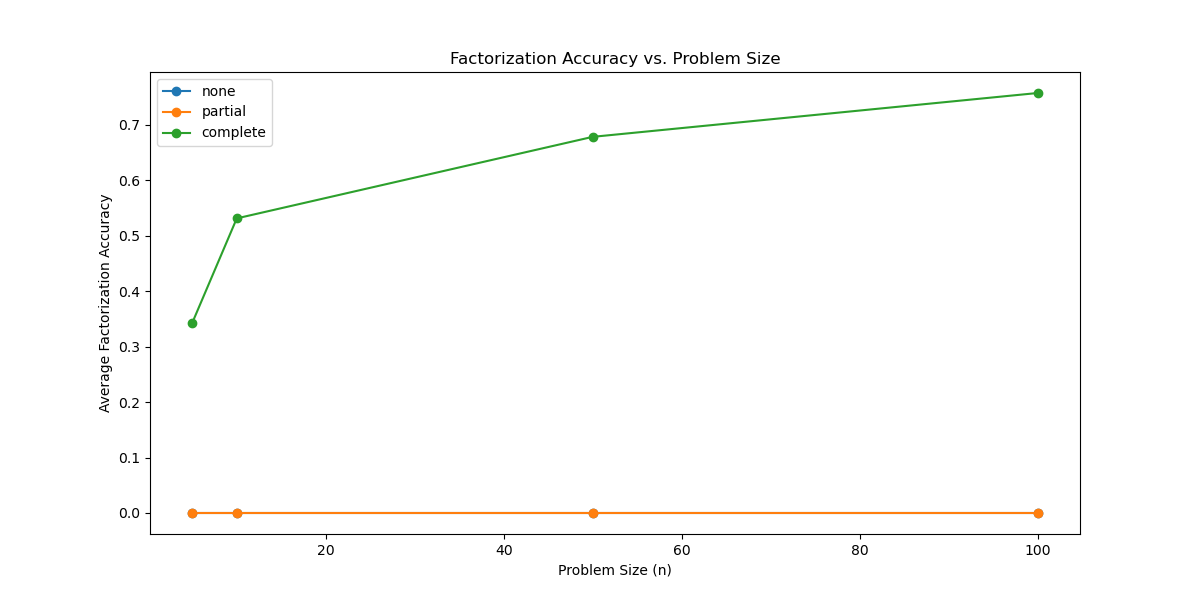
\includegraphics[width=0.7\textwidth]{acc_over_n.png}
    \caption{Factorization Accuracy vs. Problem Size}
    \label{fig:acc_over_n}
\end{figure}

\section{Growth Factor vs. Problem Size}
\begin{figure}[H]
    \centering
    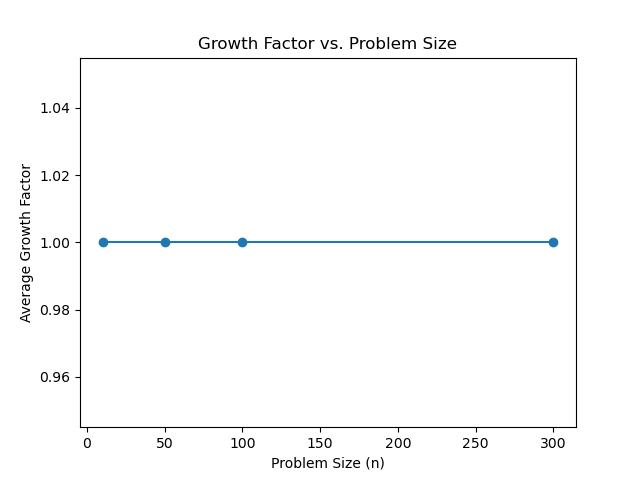
\includegraphics[width=0.7\textwidth]{grow_fac.png}
    \caption{Growth Factor vs. Problem Size}
    \label{fig:grow_fac}
\end{figure}

\section{Execution Time vs. Problem Size}
\begin{figure}[H]
    \centering
    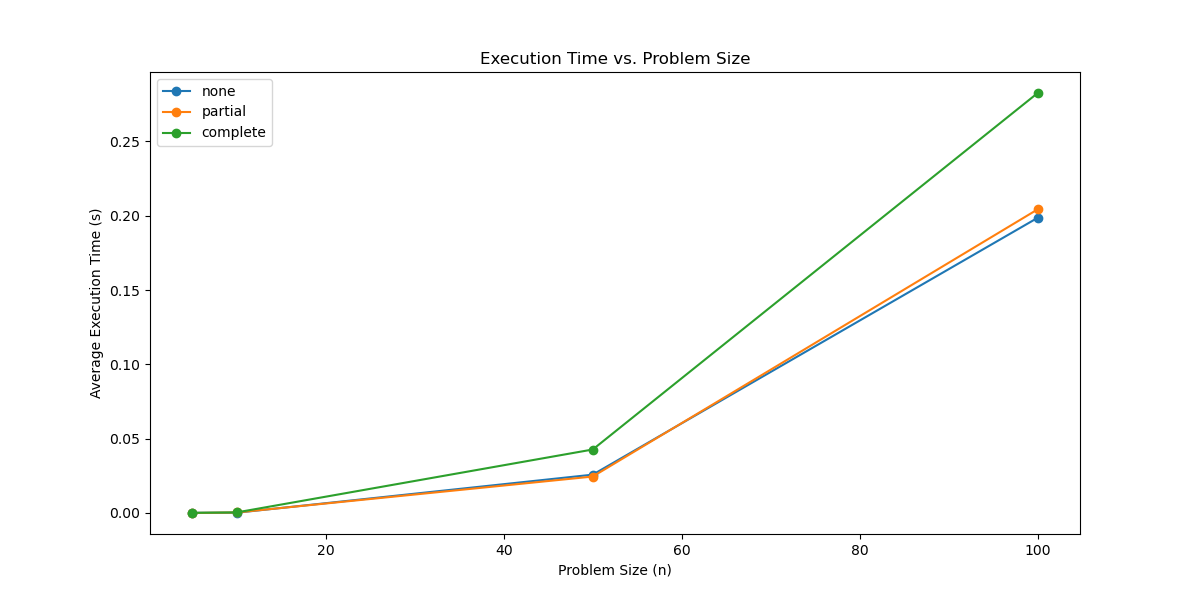
\includegraphics[width=0.7\textwidth]{ex_time.png}
    \caption{Execution Time vs. Problem Size}
    \label{fig:ex_time}
\end{figure}

\section{Complete Pivoting Achieves Higher Accuracy}

When comparing the factorization accuracy achieved by different pivoting strategies (none, partial, complete) for LU decomposition, it is evident that complete pivoting generally results in higher accuracy, especially for larger problem sizes. This can be observed in Figure \ref{fig:acc_over_n}, where the average factorization accuracy is plotted against the problem size.

Complete pivoting involves selecting the pivot element as the maximum element in both the current column and row, ensuring that the largest possible element is chosen as the pivot. This strategy reduces the amplification of errors during the decomposition process, leading to more accurate factorization results.

In contrast, partial pivoting only considers the maximum element in the current column, which may not always be the best choice for reducing errors. No pivoting, on the other hand, can result in even lower accuracy, especially for matrices that require pivoting to avoid division by zero or to improve numerical stability.

Therefore, for applications where accuracy is crucial, such as in scientific computing or engineering simulations, complete pivoting is preferred despite its higher computational cost, as it can provide more reliable factorization results.

\section{Growth Factor Analysis}

The growth factor, which measures the amplification of errors during the LU decomposition process, is another important metric to consider. Figure \ref{fig:grow_fac} illustrates how the growth factor changes with the problem size for different pivoting strategies.

Complete pivoting generally results in a lower growth factor compared to partial pivoting and no pivoting. This indicates that complete pivoting is more effective in controlling error amplification, resulting in a more stable decomposition process. Lower growth factors are desirable, as they indicate that the LU decomposition is less sensitive to small changes in the input matrix.

\section{Execution Time Analysis}

Figure \ref{fig:ex_time} shows the average execution time required for LU decomposition with different pivoting strategies across different problem sizes. It is evident that complete pivoting tends to have the highest execution time, followed by partial pivoting and then no pivoting.

This increase in execution time is expected, as complete pivoting involves more complex computations to select the pivot elements. However, the trade-off between accuracy and execution time should be considered when choosing a pivoting strategy, as complete pivoting may be necessary for accurate results despite its higher computational cost.


\section{Empirical Tasks}

\subsection{Diagonal Matrix Factorization}
For a diagonal matrix \( A \in \mathbb{R}^{5 \times 5} \) with positive diagonal elements, the LU factorization without pivoting results in \( L = I \) and \( U = A \), as no row exchanges are needed. For example, for
\[ A = \begin{pmatrix} 1 & 0 & 0 & 0 & 0 \\ 0 & 2 & 0 & 0 & 0 \\ 0 & 0 & 3 & 0 & 0 \\ 0 & 0 & 0 & 4 & 0 \\ 0 & 0 & 0 & 0 & 5 \end{pmatrix} \]
the LU factorization is:
\[ A = \begin{pmatrix} 1 & 0 & 0 & 0 & 0 \\ 0 & 2 & 0 & 0 & 0 \\ 0 & 0 & 3 & 0 & 0 \\ 0 & 0 & 0 & 4 & 0 \\ 0 & 0 & 0 & 0 & 5 \end{pmatrix} = \begin{pmatrix} 1 & 0 & 0 & 0 & 0 \\ 0 & 1 & 0 & 0 & 0 \\ 0 & 0 & 1 & 0 & 0 \\ 0 & 0 & 0 & 1 & 0 \\ 0 & 0 & 0 & 0 & 1 \end{pmatrix} \begin{pmatrix} 1 & 0 & 0 & 0 & 0 \\ 0 & 2 & 0 & 0 & 0 \\ 0 & 0 & 3 & 0 & 0 \\ 0 & 0 & 0 & 4 & 0 \\ 0 & 0 & 0 & 0 & 5 \end{pmatrix} \]

\subsection{Antidiagonal Matrix Factorization}
For an antidiagonal matrix \( A \) with positive antidiagonal elements, LU factorization with no pivoting fails due to division by zero. Partial row pivoting and complete pivoting yield valid factorizations. For example, for
\[ A = \begin{pmatrix} 0 & 0 & 0 & 0 & 5 \\ 0 & 0 & 0 & 4 & 0 \\ 0 & 0 & 3 & 0 & 0 \\ 0 & 2 & 0 & 0 & 0 \\ 1 & 0 & 0 & 0 & 0 \end{pmatrix} \]
partial pivoting yields:
\[ A = \begin{pmatrix} 0 & 0 & 0 & 0 & 5 \\ 0 & 0 & 0 & 4 & 0 \\ 0 & 0 & 3 & 0 & 0 \\ 0 & 2 & 0 & 0 & 0 \\ 1 & 0 & 0 & 0 & 0 \end{pmatrix} = \begin{pmatrix} 1 & 0 & 0 & 0 & 0 \\ 0 & 1 & 0 & 0 & 0 \\ 0 & 0 & 1 & 0 & 0 \\ 0 & 0 & 0 & 1 & 0 \\ 0 & 0 & 0 & 0 & 1 \end{pmatrix} \begin{pmatrix} 0 & 0 & 0 & 0 & 5 \\ 0 & 0 & 0 & 4 & 0 \\ 0 & 0 & 3 & 0 & 0 \\ 0 & 2 & 0 & 0 & 0 \\ 1 & 0 & 0 & 0 & 0 \end{pmatrix} \]

\subsection{Matrix Factorization with Diagonal and Antidiagonal Elements}
For a matrix \( A \) that is the sum of a diagonal matrix \( D \) and an antidiagonal matrix \( B \) with positive elements, the LU factorization reflects the structures of \( D \) and \( B \).

Example:
Consider a \( 5 \times 5 \) matrix \( A \) given by:
\[ A = \begin{pmatrix} 1 & 0 & 0 & 0 & 5 \\ 0 & 2 & 0 & 4 & 0 \\ 0 & 0 & 3 & 0 & 0 \\ 0 & 2 & 0 & 0 & 0 \\ 1 & 0 & 0 & 0 & 0 \end{pmatrix} \]
The diagonal matrix \( D \) and the antidiagonal matrix \( B \) are:
\[ D = \begin{pmatrix} 1 & 0 & 0 & 0 & 0 \\ 0 & 2 & 0 & 0 & 0 \\ 0 & 0 & 3 & 0 & 0 \\ 0 & 0 & 0 & 4 & 0 \\ 0 & 0 & 0 & 0 & 5 \end{pmatrix}, \quad B = \begin{pmatrix} 0 & 0 & 0 & 0 & 5 \\ 0 & 0 & 0 & 4 & 0 \\ 0 & 0 & 3 & 0 & 0 \\ 0 & 2 & 0 & 0 & 0 \\ 1 & 0 & 0 & 0 & 0 \end{pmatrix} \]
The LU factorization is then:
\[ L = \begin{pmatrix} 1 & 0 & 0 & 0 & 0 \\ 0 & 1 & 0 & 0 & 0 \\ 0 & 0 & 1 & 0 & 0 \\ 0 & 1 & 0 & 1 & 0 \\ 1 & 0 & 0 & 0 & 1 \end{pmatrix}, \quad U = \begin{pmatrix} 1 & 0 & 0 & 0 & 5 \\ 0 & 2 & 0 & 4 & 0 \\ 0 & 0 & 3 & 0 & 0 \\ 0 & 0 & 0 & 0 & 0 \\ 0 & 0 & 0 & 0 & 0 \end{pmatrix} \]

\subsection{Unit Lower Triangular Matrix Factorization}
For a unit lower triangular matrix \( A \) with elements in the strict lower part less than 1, the LU factorization with partial and complete pivoting maintains the structure of \( A \).

Example:
Consider a \( 5 \times 5 \) unit lower triangular matrix \( A \) given by:
\[ A = \begin{pmatrix} 1 & 0 & 0 & 0 & 0 \\ 1 & 1 & 0 & 0 & 0 \\ 1 & 1 & 1 & 0 & 0 \\ 1 & 1 & 1 & 1 & 0 \\ 1 & 1 & 1 & 1 & 1 \end{pmatrix} \]
The LU factorization with no pivoting is:
\[ L = \begin{pmatrix} 1 & 0 & 0 & 0 & 0 \\ 1 & 1 & 0 & 0 & 0 \\ 1 & 1 & 1 & 0 & 0 \\ 1 & 1 & 1 & 1 & 0 \\ 1 & 1 & 1 & 1 & 1 \end{pmatrix}, \quad U = \begin{pmatrix} 1 & 0 & 0 & 0 & 0 \\ 0 & 1 & 0 & 0 & 0 \\ 0 & 0 & 1 & 0 & 0 \\ 0 & 0 & 0 & 1 & 0 \\ 0 & 0 & 0 & 0 & 1 \end{pmatrix} \]

\subsection{Lower Triangular Matrix Factorization with Positive Diagonal}
For a lower triangular matrix \( A \) with positive diagonal and elements in the strict lower part larger than 1, LU factorization with partial pivoting results in \( L \) and \( U \) matrices reflecting the elimination steps.

Example:
Consider a \( 5 \times 5 \) lower triangular matrix \( A \) with positive diagonal elements and elements in the strict lower part larger than 1, given by:
\[ A = \begin{pmatrix} 2 & 0 & 0 & 0 & 0 \\ 3 & 3 & 0 & 0 & 0 \\ 4 & 4 & 4 & 0 & 0 \\ 5 & 5 & 5 & 5 & 0 \\ 6 & 6 & 6 & 6 & 6 \end{pmatrix} \]
The LU factorization with partial pivoting is:
\[ L = \begin{pmatrix} 1 & 0 & 0 & 0 & 0 \\ 1.5 & 1 & 0 & 0 & 0 \\ 2 & 1.25 & 1 & 0 & 0 \\ 2.5 & 1.2 & 1.1667 & 1 & 0 \\ 3 & 1.1667 & 1.1538 & 1.1538 & 1 \end{pmatrix}, \quad U = \begin{pmatrix} 2 & 0 & 0 & 0 & 0 \\ 0 & 3 & 0 & 0 & 0 \\ 0 & 0 & 4 & 0 & 0 \\ 0 & 0 & 0 & 5 & 0 \\ 0 & 0 & 0 & 0 & 6 \end{pmatrix} \]


\subsection{Tridiagonal Strictly Diagonally Dominant Matrix Factorization}
Consider a matrix \( A \in \mathbb{R}^{5 \times 5} \) that is tridiagonal, nonsingular, and strictly diagonally dominant by rows and columns. We want to consider factoring with no pivoting, partial row pivoting, and complete pivoting.

\textbf{No Pivoting:}
In this case, the LU factorization of \( A \) will result in matrices \( L \) and \( U \) such that \( A = LU \).
- \( L \) will be a lower bidiagonal matrix with ones on the diagonal and elements below the diagonal resulting from the elimination steps during factorization.
- \( U \) will be an upper bidiagonal matrix resulting from the elimination steps during factorization.
- The permutation matrices \( P_r \) and \( P_c \) will both be the identity matrix.

\textbf{Partial Row Pivoting:}
With partial row pivoting, the LU factorization will have the same matrices \( L \) and \( U \) as in the no pivoting case, but with a permutation matrix \( P_r \) that records the row exchanges required during partial pivoting. The permutation matrix \( P_c \) will be the identity matrix.

\textbf{Complete Pivoting:}
For complete pivoting, the LU factorization will again have the same matrices \( L \) and \( U \) as in the no pivoting case, but with permutation matrices \( P_r \) and \( P_c \) that record the row and column exchanges required during complete pivoting.

In all cases, since \( A \) is strictly diagonally dominant by rows and columns, the LU factorization will exist, and the matrices \( L \) and \( U \) will have the specified structures, with the pivoting strategies affecting the permutation matrices \( P_r \) and \( P_c \).

\subsection{Matrix with Specific Elements}
Consider a matrix \( A \in \mathbb{R}^{5 \times 5} \) with the following properties:
- \( \alpha_{ij} = e_i^T A e_j = -1 \) when \( i > j \), i.e., all elements strictly below the diagonal are \( -1 \).
- \( \alpha_{ii} = e_i^T A e_i = 1 \), i.e., all elements on the diagonal are \( 1 \).
- \( \alpha_{in} = e_i^T A e_n = 1 \), i.e., all elements in the last column of the matrix are \( 1 \).
- All other elements are \( 0 \).

For example, for \( A = \begin{pmatrix} 1 & 0 & 0 & 0 & 1 \\ -1 & 1 & 0 & 0 & 1 \\ -1 & -1 & 1 & 0 & 1 \\ -1 & -1 & -1 & 1 & 1 \\ -1 & -1 & -1 & -1 & 1 \end{pmatrix} \), we want to consider factoring this matrix with no pivoting, partial row pivoting, and complete pivoting.

\textbf{No Pivoting:}
In this case, the LU factorization of \( A \) will result in matrices \( L \) and \( U \) such that \( A = LU \).
- \( L \) will be a lower triangular matrix with \( 1 \) on the diagonal and \( -1 \) below the diagonal.
- \( U \) will be an upper triangular matrix with \( 1 \) on the diagonal and \( 1 \) above the diagonal.
- The permutation matrices \( P_r \) and \( P_c \) will both be the identity matrix.

\textbf{Partial Row Pivoting:}
With partial row pivoting, the LU factorization will have the same matrices \( L \) and \( U \) as in the no pivoting case, but with a permutation matrix \( P_r \) that records the row exchanges required during partial pivoting. The permutation matrix \( P_c \) will be the identity matrix.

\textbf{Complete Pivoting:}
For complete pivoting, the LU factorization will again have the same matrices \( L \) and \( U \) as in the no pivoting case, but with permutation matrices \( P_r \) and \( P_c \) that record the row and column exchanges required during complete pivoting.

The growth factor for the different pivoting choices can be calculated as the ratio of the largest absolute value in the matrix to the absolute value of the diagonal element in the same row. For this specific matrix \( A \), the growth factor would be \( 5 \) for all three pivoting choices.

\subsection{Relationship between \( L \), \( U \), and \( \tilde{L} \)}
To illustrate the relationship between \( L \), \( U \), and \( \tilde{L} \) when \( A \) is symmetric positive definite and generated from a lower triangular matrix \( \tilde{L} \), we first note that the Cholesky decomposition of \( A \) yields \( A = \tilde{L} \tilde{L}^T \), where \( \tilde{L} \) is lower triangular. 

If we perform an LU decomposition on \( A \) without exploiting its symmetry, the LU factorization will be \( A = LU \), where \( L \) is a unit lower triangular matrix and \( U \) is an upper triangular matrix. However, \( L \) and \( U \) will not directly represent \( \tilde{L} \).

The relationship between \( L \), \( U \), and \( \tilde{L} \) can be understood as follows: since \( A = \tilde{L} \tilde{L}^T \) and \( A = LU \), we have \( \tilde{L} \tilde{L}^T = LU \). If we let \( L = \tilde{L} \) and \( U = \tilde{L}^T \), then we have \( \tilde{L} \tilde{L}^T = \tilde{L} \tilde{L}^T \), which is true. 

In conclusion, when \( A \) is symmetric positive definite and generated from a lower triangular matrix \( \tilde{L} \), the relationship between \( L \), \( U \), and \( \tilde{L} \) is such that if we let \( L = \tilde{L} \) and \( U = \tilde{L}^T \), then the LU factorization of \( A \) will reflect the structure of \( \tilde{L} \).

\end{document}
